\chapter{Methodology}
\label{ch:methodology}

This chapter outlines the methodology used in this study, which draws inspiration from the \citetitle{STraTS2022} by \citeauthor{STraTS2022} \cite{STraTS2022}. We aim to extend their approach to address the challenges of mortality prediction using clinical time-series data. The model leverages a transformer-based architecture to generate robust representations of patient data, following a pretraining and fine-tuning strategy.

We begin by presenting the backbone network architecture in \cref{sec:backbone}, which forms the core of our model. The pretraining phase, described in \cref{sec:pretraining}, introduces a self-supervised task where the model learns temporal dynamics through forecasting. The fine-tuning phase in \cref{sec:finetuning} then adapts the pretrained model for mortality prediction.

In subsequent sections, we discuss the training procedure (\cref{sec:training_procedure}), and the implementation details (\cref{sec:implementation_details}). Finally, we compare our approach with several baseline methods in \cref{sec:baselines} and describe the experimental setup in \cref{sec:experiments}.

\paragraph{Notations}

Throughout this chapter, we refer to the ``event'' entities of a \gls{mimiciii} dataset as ``observations'' to maintain consistency with the terminology of the original paper. Furthermore, in this and subsequent chapters we may refer to \textit{fine-tuning stage}, \textit{mortality prediction}, and \textit{time series classification} interchangeably, depending on the context. Similarly, the terms \textit{pretraining stage} and \textit{time series forecasting} can be used interchangeably. Lastly, \cref{tab:model_notations} summarizes the mathematical notations used in this chapter.

\begin{table}[h!]
    \centering
    \caption{Notations used in this section}
    \label{tab:model_notations}
    \begin{tabular}{ll}
\toprule
\textbf{Notation} & \textbf{Definition} \\
\midrule
\(t_i \in \mathbb{R}_{\geq 0}\) & Time of \(i\)th observation \\
\(f_i \in \mathcal{F}\) & Clinical variable of \(i\)th observation \\
\(v_i \in \mathbb{R}\) & Value of \(i\)th observation \\
\(\bar{t}_i, \bar{v}_i\) & Normalized time and value \\
\(\mathbf{T}\) & Multivariate time series \(\{(t_i, f_i, v_i)\}_{i=1}^n\) \\
\(\mathbf{e}_i^f, \mathbf{e}_i^v, \mathbf{e}_i^t \in \mathbb{R}^d\) & Feature, value and time embeddings for \(f_i\) \\
\(\mathbf{e}_i \in \mathbb{R}^d = \mathbf{e}_i^f + \mathbf{e}_i^v + \mathbf{e}_i^t\) & Initial triplet embedding for \(i\)th observation \\
\(\mathbf{E} \in \mathbb{R}^{n \times d}\) & Sequence of triplet embeddings \\
\(\mathbf{C} \in \mathbb{R}^{n \times d}\) & Contextual triplet embeddings \\
\(\alpha_i\) & Attention weight for \(i\)th contextual embedding \\
\(\mathbf{e}^T \in \mathbb{R}^d\) & Time-series embedding \\
\(\mathbf{d} \in \mathbb{R}^D\) & Demographics vector \\
\(\mathbf{e}^d \in \mathbb{R}^d\) & Demographics embedding \\
\(\mathbf{W}_\cdot \in \mathbb{M}\) & Weight matrix \\
\(\mathbf{b}_\cdot \in \mathbb{R}^d\) & Bias vector \\
\(\mathcal{M}, \mathcal{M}_{pt}, \mathcal{M}_{ft}\) & Backbone, pretrained and fine-tuned models \\
\(\mathcal{D}_{\text{split}}, \mathcal{D}'_{\text{split}} \) & Pretraining and fine-tuning datasets for corresponding splits \\
\bottomrule
\end{tabular}

\end{table}

\section{Backbone Network Architecture}
\label{sec:backbone}

In this section, we present the architecture of the backbone model, denoted as \(\mathcal{M}\). The term \textit{backbone} is commonly used in the context of neural networks to refer to the core components of a model that serve as the foundation for subsequent tasks. This backbone model is responsible for generating vector representations (embeddings) from multivariate time-series data, which include both clinical variables and demographic information. This backbone model serves as a \emph{feature extractor}, transforming raw input data into meaningful vector representations.

The architecture described here is \emph{headless}, which means that it excludes the final task-specific layers (or \emph{heads}) typically used for classification or regression. Instead, \(\mathcal{M}\) focuses on producing robust vector embeddings that encapsulate the intricacies of a patient's journey through their \gls{icu} stay. These embeddings can be subsequently fed into various heads, each tailored for specific downstream tasks, such as mortality prediction, length-of-stay estimation, or other clinically relevant outcomes.

The following subsections provide a detailed description of the main components of the backbone model, closely following the structure and notations presented in the original paper.

\subsection{Continuous Value Embedding}
\label{sec:cve}

In their work, \citeauthor{STraTS2022} proposed a \gls{cve} technique using a one-to-many \gls{ffn} with learnable parameters, defined as
\[ \mathbf{e} = \text{FFN}(v) \in \mathbb{R}^d. \]

The \gls{ffn} has one input neuron and \(d\) output neurons, with a single hidden layer containing \(\lfloor \sqrt{d} \rfloor\) neurons and a \(\tanh(\cdot)\) activation function. Formally, it is expressed as:
\[
\text{FFN}(x) = U \tanh(Wx + b),
\]
where \(W \in \mathbb{R}^{\lfloor \sqrt{d} \rfloor \times 1}\), \(b \in \mathbb{R}^{\lfloor \sqrt{d} \rfloor}\), and \(U \in \mathbb{R}^{d \times \lfloor \sqrt{d} \rfloor}\). Unlike commonly used sinusoidal encodings with a fixed set of frequencies, this technique offers more flexibility by allowing end-to-end learning of continuous value embeddings without the need to categorize the input values.

\subsection{Initial Triplet Embedding}

Given an input time series \( \mathbf{T} = \{(t_i, f_i, v_i)\}_{i=1}^n \), where each observation triplet consists of the time \(t_i \in \mathbb{R}_{\geq 0}\), the feature \(f_i \in \mathcal{F}\), and the corresponding value \(v_i \in \mathbb{R}\), the model computes an initial triplet embedding \(\mathbf{e}_i \in \mathbb{R}^d\).

The initial triplet embedding \(\mathbf{e}_i\) is obtained by summing three component embeddings:

\begin{itemize}
    \item \textbf{Feature Embedding} \(\mathbf{e}_i^f \in \mathbb{R}^d\): Maps each feature \(f_i\) to a learnable embedding vector.
    \item \textbf{Value Embedding} \(\mathbf{e}_i^v \in \mathbb{R}^d\): Computed using the \gls{cve} technique applied to the observed value \(v_i\).
    \item \textbf{Time Embedding} \(\mathbf{e}_i^t \in \mathbb{R}^d\): Computed using the \gls{cve} technique applied to the observation time \(t_i\).
\end{itemize}

This step is summarized as:
\[
\mathbf{e}_i = \mathbf{e}_i^f + \mathbf{e}_i^v + \mathbf{e}_i^t.
\]

\subsection{Contextual Triplet Embedding}

The sequence of initial embeddings \(\mathbf{E} = [\mathbf{e}_1, \ldots, \mathbf{e}_n] \in \mathbb{R}^{n \times d}\) is passed through a transformer model composed of \(M\) blocks. Each block includes a \gls{mha} layer with \(h\) attention heads, followed by a \gls{ffn} with a single hidden layer.

The computation for the \(j\)-th attention head in the \gls{mha} layer is given by:
\[
H_j = \text{Softmax}\left(\frac{\mathbf{E} \mathbf{W}^q_j (\mathbf{E} \mathbf{W}^k_j)^\top}{\sqrt{d / h}}\right) \mathbf{E} \mathbf{W}^v_j, \quad \text{for} \quad j = 1, \ldots, h,
\]
where \(\mathbf{W}^q_j, \mathbf{W}^k_j, \mathbf{W}^v_j \in \mathbb{R}^{d \times \lfloor d / h \rfloor}\) are the query, key and value projection matrices for the \(j\)-th head.

The outputs of all attention heads are concatenated and projected as:
\[
\text{MHA}(\mathbf{E}) = \left[ H_1 \, \Vert \, \cdots \, \Vert \, H_h \right] \mathbf{W}_o,
\]
where \(\mathbf{W}_o \in \mathbb{R}^{d \times d}\) is the output projection matrix.

The \gls{ffn} layer is defined as:
\[
\text{FFN}(\mathbf{X}) = \text{GELU}(\mathbf{X} \mathbf{W}_1^f + \mathbf{b}_1^f) \mathbf{W}_2^f + \mathbf{b}_2^f,
\]
where \(\mathbf{W}_1^f \in \mathbb{R}^{d \times 2d}\), \(\mathbf{W}_2^f \in \mathbb{R}^{2d \times d}\), and biases \(\mathbf{b}_1^f \in \mathbb{R}^{2d}\), \(\mathbf{b}_2^f \in \mathbb{R}^d\).

The Gaussian Error Linear Unit (GELU) \cite{gelu} is an activation function defined as:
\[
\text{GELU}(x) = x \cdot \Phi(x),
\]
where \( \Phi(x) \) is the \gls{cdf} of the standard normal distribution.

One key advantage of GELU is that it introduces nonlinearity even in the negative domain, unlike ReLU, which sets negative values to zero. Furthermore, GELU is differentiable across the entire input domain, whereas ReLU is not differentiable at zero. This smoothness improves the model optimization by gradient descent, providing more stability during training.

The output of the transformer, denoted as \(\mathbf{C} = [\mathbf{c}_1, \dots, \mathbf{c}_n]^\top \in \mathbb{R}^{n \times d}\), captures the contextual dependencies among the triplets. It is computed using residual connections in a post-norm architecture as follows:

\[
\mathbf{A} = \text{LayerNorm}_1\left(\text{MHA}(\mathbf{E}) + \mathbf{E}\right),
\]
\[
\mathbf{C} = \text{LayerNorm}_2\left(\text{FFN}(\mathbf{A}) + \mathbf{A}\right)
\]

where \(\text{LayerNorm}_1\) and \(\text{LayerNorm}_2\) are layer normalization functions applied to the output of the \gls{mha} and \gls{ffn} layers, respectively.

\subsection{Fusion Self-Attention}
\label{sec:fusion_self_attention}

To integrate the contextual embeddings into a unified time-series representation, a self-attention mechanism inspired by those used in natural language processing is employed. This mechanism allows the model to weigh the importance of each contextual embedding \(\mathbf{c}_i\) when forming the overall time-series embedding \(\mathbf{e}^T\).

First, an attention score \(a_i\) is computed for each contextual embedding:

\[
a_i = \mathbf{u}_a^\top \tanh(\mathbf{W}_a \mathbf{c}_i + \mathbf{b}_a),
\]

where $\mathbf{W}_a\in \mathbb{R}^{d \times d}, \mathbf{b}_a\in\mathbb{R}^{d}, \mathbf{u_a}\in\mathbb{R}^{d}$ are the weights of this fusion attention network.

Next, the attention scores are converted into normalized weights using the softmax function:

\[
\alpha_i = \frac{\exp(a_i)}{\sum_{j=1}^{n} \exp(a_j)}.
\]

The attention weights \(\alpha_i\) reflect the relative importance of each time step in the sequence.

Finally, the time-series embedding is computed as a weighted sum of the contextual embeddings:

\[
\mathbf{e}^T = \sum_{i=1}^{n} \alpha_i \mathbf{c}_i.
\]

This process aggregates the entire sequence into a single vector, emphasizing the most relevant observations based on the learned attention weights.

\subsection{Demographics Embedding}
\label{sec:demographics_embedding}

Demographic information \(\mathbf{d} \in \mathbb{R}^D\) is incorporated into the model through a separate embedding process. The demographics embedding \(\mathbf{e}^d \in \mathbb{R}^d\) is computed by passing \(\mathbf{d}\) through a \gls{ffn}:
\[
\mathbf{e}^d = \mathbf{W}_1^d \tanh\left( \mathbf{W}_2^d \mathbf{d} + \mathbf{b}_2^d \right) + \mathbf{b}_1^d,
\]
where \(\mathbf{W}_1^d \in \mathbb{R}^{d \times 2d}\), \(\mathbf{W}_2^d \in \mathbb{R}^{2d \times D}\), \(\mathbf{b}_1^d \in \mathbb{R}^{d}\), and \(\mathbf{b}_2^d \in \mathbb{R}^{2d}\) are learnable parameters. This process resembles the \gls{cve} technique, with the primary difference being the size of the hidden layer and number of input neurons.


\subsection{Integrated Vector Representation}

The backbone network generates embeddings for both clinical time-series data and demographic information. The final output of the backbone network is a concatenated vector representation that integrates these embeddings.

Formally, the complete embedding produced by the model is expressed as:
\[
\mathcal{M}(\mathbf{T}, \mathbf{d}) = \mathbf{e}^d \Vert \mathbf{e}^T,
\]
where \( \mathbf{e}^d \) represents the demographics embedding and \( \mathbf{e}^T \) denotes the time-series embedding. This integrated representation \( \mathcal{M} \) serves as the input for subsequent model components, which are tailored to different downstream tasks such as forecasting or classification.


By integrating the embeddings of clinical time-series data and demographic information, the backbone network produces a vector representation that captures both temporal dynamics and patient characteristics.

\section{Training Procedure}
\label{sec:training_procedure}

In this section, we outline the training procedure employed to develop our model, including data preprocessing, optimization configurations, and model selection strategies.

\subsection{Data Preprocessing}

The training process begins with data loading and preprocessing. We apply Z-score normalization to standardize the values in observation triplets and the age, ensuring that each has a mean of zero and a standard deviation of one. This standardization is beneficial when dealing with features of varying scales, as it ensures that each feature have similar scale and magnitude and thus contributes equally to the model's learning process.

The standardized value \( \bar{v} \) for a feature \( f \) is calculated as:

\[
\bar{v} = \frac{v - \mu_f}{\sigma_f},
\]

where \( v \) is the original value, \( \mu_f \) is the mean, and \( \sigma_f \) is the standard deviation of feature \( f \) computed from the training data.

\subsubsection*{Variable Dropout}
\label{sec:variable_dropout}

Variable dropout is a form of data augmentation that involves randomly dropping out a subset of features (variables) from the input sequence during training. This technique helps prevent overfitting by encouraging the model to learn robust representations that do not rely on any single feature \cite{DropoutSimpleWay2014}. By simulating missing features during prediction, this technique improves the model's ability to handle incomplete data in real-world applications.

Specifically, we exclude a random subset of features from the entire input sequence with a probability \(p = 0.2\), meaning that for each feature \(f_i\), we decide whether to drop it across all time steps. This process is formally expressed as:
\begin{equation}
    \label{eq:variable_dropout}
    \mathbf{T}' = \left\{ (t_i, f_i, v_i) \in \mathbf{T} \,\big|\, r_{f_i} = 1 \right\}, \quad \text{where } r_{f_j} \sim \text{Bernoulli}(1 - p), j = 1, \dots, |\mathcal{F}|.
\end{equation}

Here, \(\mathbf{T}\) represents the original set of events, and \(r_{f_i}\) is a binary variable indicating whether feature \(f_i\) is retained (\(r_{f_i} = 1\)) or dropped (\(r_{f_i} = 0\)). The modified time series  \(\mathbf{T}'\) thus consists only of a subset of retained feature observations.

\subsection{Optimization Configuration}

The optimization process involves configuring the training parameters to efficiently minimize the loss function. Key components include the choice of optimizer, batch size, learning rate, and regularization techniques.

\subsubsection{AdamW Optimizer}

We utilize the AdamW optimizer \cite{DecoupledWeightDecay2019}, an extension of the Adam optimizer that decouples weight decay from the gradient update rule. Weight decay, a form of L2 regularization, helps prevent overfitting by penalizing large weight values. In AdamW, weight decay is applied directly to the model weights, which typically results in better generalization performance.

The update rule for AdamW is:

\[
\theta_{t+1} = \theta_t - \eta \left( \frac{m_t}{\sqrt{v_t} + \epsilon} + \lambda \theta_t \right),
\]

where \(\theta_t\) represents the model parameters at time \(t\), \(\eta\) is the learning rate, \(m_t\) and \(v_t\) are the first and second moment estimates of the gradients, \(\epsilon\) is a small constant to prevent division by zero, and \(\lambda\) is the weight decay coefficient.

In contrast to the original study, we disabled weight decay for the norm and bias parameters. This is a common practice in deep learning because applying weight decay to these parameters can be counterproductive\cite{BagTricksImage2018}.

\subsubsection{Batch Size and Learning Rate}

We use a batch size of \num{16} for both pretraining and fine-tuning stages, balancing computational efficiency and gradient estimation stability.

The learning rate is set to \(1 \times 10^{-4}\) during pretraining and reduced to \(1 \times 10^{-5}\) during fine-tuning. A smaller learning rate in the fine-tuning phase allows for more precise updates and helps prevent divergence from the pretrained parameters.

\subsection{Model Selection}

Model selection involves evaluating and choosing the model configuration that best generalizes to unseen data. We employ validation and early stopping strategies to prevent overfitting and select optimal model parameters.

We use a validation set, distinct from the training data, to monitor the model's performance during training. After each epoch, the model is evaluated on the validation set using the defined evaluation metrics. This process provides insights into the model's generalization ability and helps detect overfitting.

Early stopping is implemented to halt training when the model's performance on the validation set ceases to improve. Specifically, if no improvement is observed in the validation loss after 10 epochs, known as the \emph{patience} parameter, training is stopped and the model with the best validation performance is restored.

\section{Pretraining Phase}
\label{sec:pretraining}

The pretraining phase aims to improve the model's ability to learn general temporal dynamics in clinical time-series data without relying on limited labeled samples. This phase enables the model to develop robust embeddings from unlabeled data, which are later fine-tuned for specific tasks, such as mortality prediction. In the referenced study, pretraining on a self-supervised forecasting task was shown to improve the final model's performance (\gls{auroc} \( +0.01 \), \gls{aucpr} \( +0.03 \). \gls{minrp} \( +0.02 \)).
\citeauthor{STraTS2022} concluded that the model pretraining ``enables learning generalized vector representations in the presence of limited labeled data and alleviates sensitivity to noise''.

In this section, we describe the data \( \mathcal{D} \), model \( \mathcal{M}_{pt} \) and the loss function used for optimizing the model during this phase.


\subsection{Unlabeled Data}

The model utilizes a dataset \( \mathcal{D} = \{(\mathbf{d}_i, \mathbf{T}_i, \mathbf{m}_i, \mathbf{z}_i)\}_{i=1}^{N} \), where \( N \) is the number of samples (i.e., \gls{icu} stays). The input time series \( \mathbf{T}_i = \{(v_j, t_j, f_j)\}_{j=1}^{n} \) is represented by three vectors of equal length: \( \mathbf{v} \) for feature values, \( \mathbf{t} \) for corresponding timestamps, and \( \mathbf{f} \) for feature identifiers.

The input time series consists of observation triplets within a random \qtyrange{12}{24}{\hour}  window, defined by the interval \([t_0, t_1]\), where \( t_1 \in [\qty{12}{\hour}; t_n ) \) is chosen randomly such that window is at least \qty{12}{\hour} and at least a single observation falls within prediction window. The start time is then \( t_0 = \max(t_1 - \qty{24}{\hour}, \qty{0}{\hour}) \).

To facilitate model training, the time values are normalized to the interval \([-1, 1]\):
\begin{equation}
    \label{eq:normalize_time}
    \bar{t}_j = \frac{t_j - t_0}{\qty{12}{\hour}} - 1 \in [-1, 1] \quad j = 1, \dots, n,
\end{equation}
where \( n \) is the number of observations in the time series.

Thus, the selected \qtyrange{12}{24}{\hour} time series is defined as:
\begin{equation}
    \label{eq:input_24_window}
    \mathbf{T}_{\qty{24}{\hour}} = \left\{ \left( \bar{t}_j, \, f_j, \, \bar{v}_j \right) \ \middle|\ t_0 \leq t_j \leq t_1 \right\}_{j = 1}^{n}.
\end{equation}

The selected time series then undergoes random variable dropout, as described in \cref{sec:variable_dropout}, to simulate missing features in the input sequence. To limit the memory requirements of the model, we the number of observations in a time series is limited to a maximum of \num{880}. If the number of observations within the time window exceeds this limit, random observations are removed to reduce the sequence length.

The model's predictions are defined as a vector of average observed values within a \qty{2}{\hour} prediction window, computed as follows:
\begin{equation}
    \label{eq:forecast_target}
    \mathbf{z}_i = \frac{1}{\| \mathbf{v}_{i,f} \|_0 } \sum^{t_2}_{t=t_1} v_{i,t,f} \in \mathbb{R}^{|\mathcal{F}|},
\end{equation}
where \( t_2 = t_1 + \qty{2}{\hour} \) is the end of the prediction window, \( v_{i,t,f} \) is the value of feature \( f \) at time \( t \), and \( \| \mathbf{v}_{i,f} \|_0 \) is the number of times feature \( f \) was observed within the prediction window.

The corresponding forecast mask \( \mathbf{m}_i \in \{0, 1\}^{|\mathcal{F}|} \) indicates which features were observed at least once during the prediction window. This mask is used to exclude unobserved features from the training process by masking them out during loss computation.

This approach allows the model to leverage both labeled and unlabeled time-series data by selecting different observation windows, thereby increasing the dataset's diversity and size. The upper part of \cref{fig:model_input} illustrates the construction of inputs for the forecasting task. The input structure consists of the three vectors, along with the demographic values \( \mathbf{d} \). The forecast mask \( \mathbf{m} \) and target values \( \mathbf{z} \) are used to compute the loss during training.


\begin{figure}
    \centering
    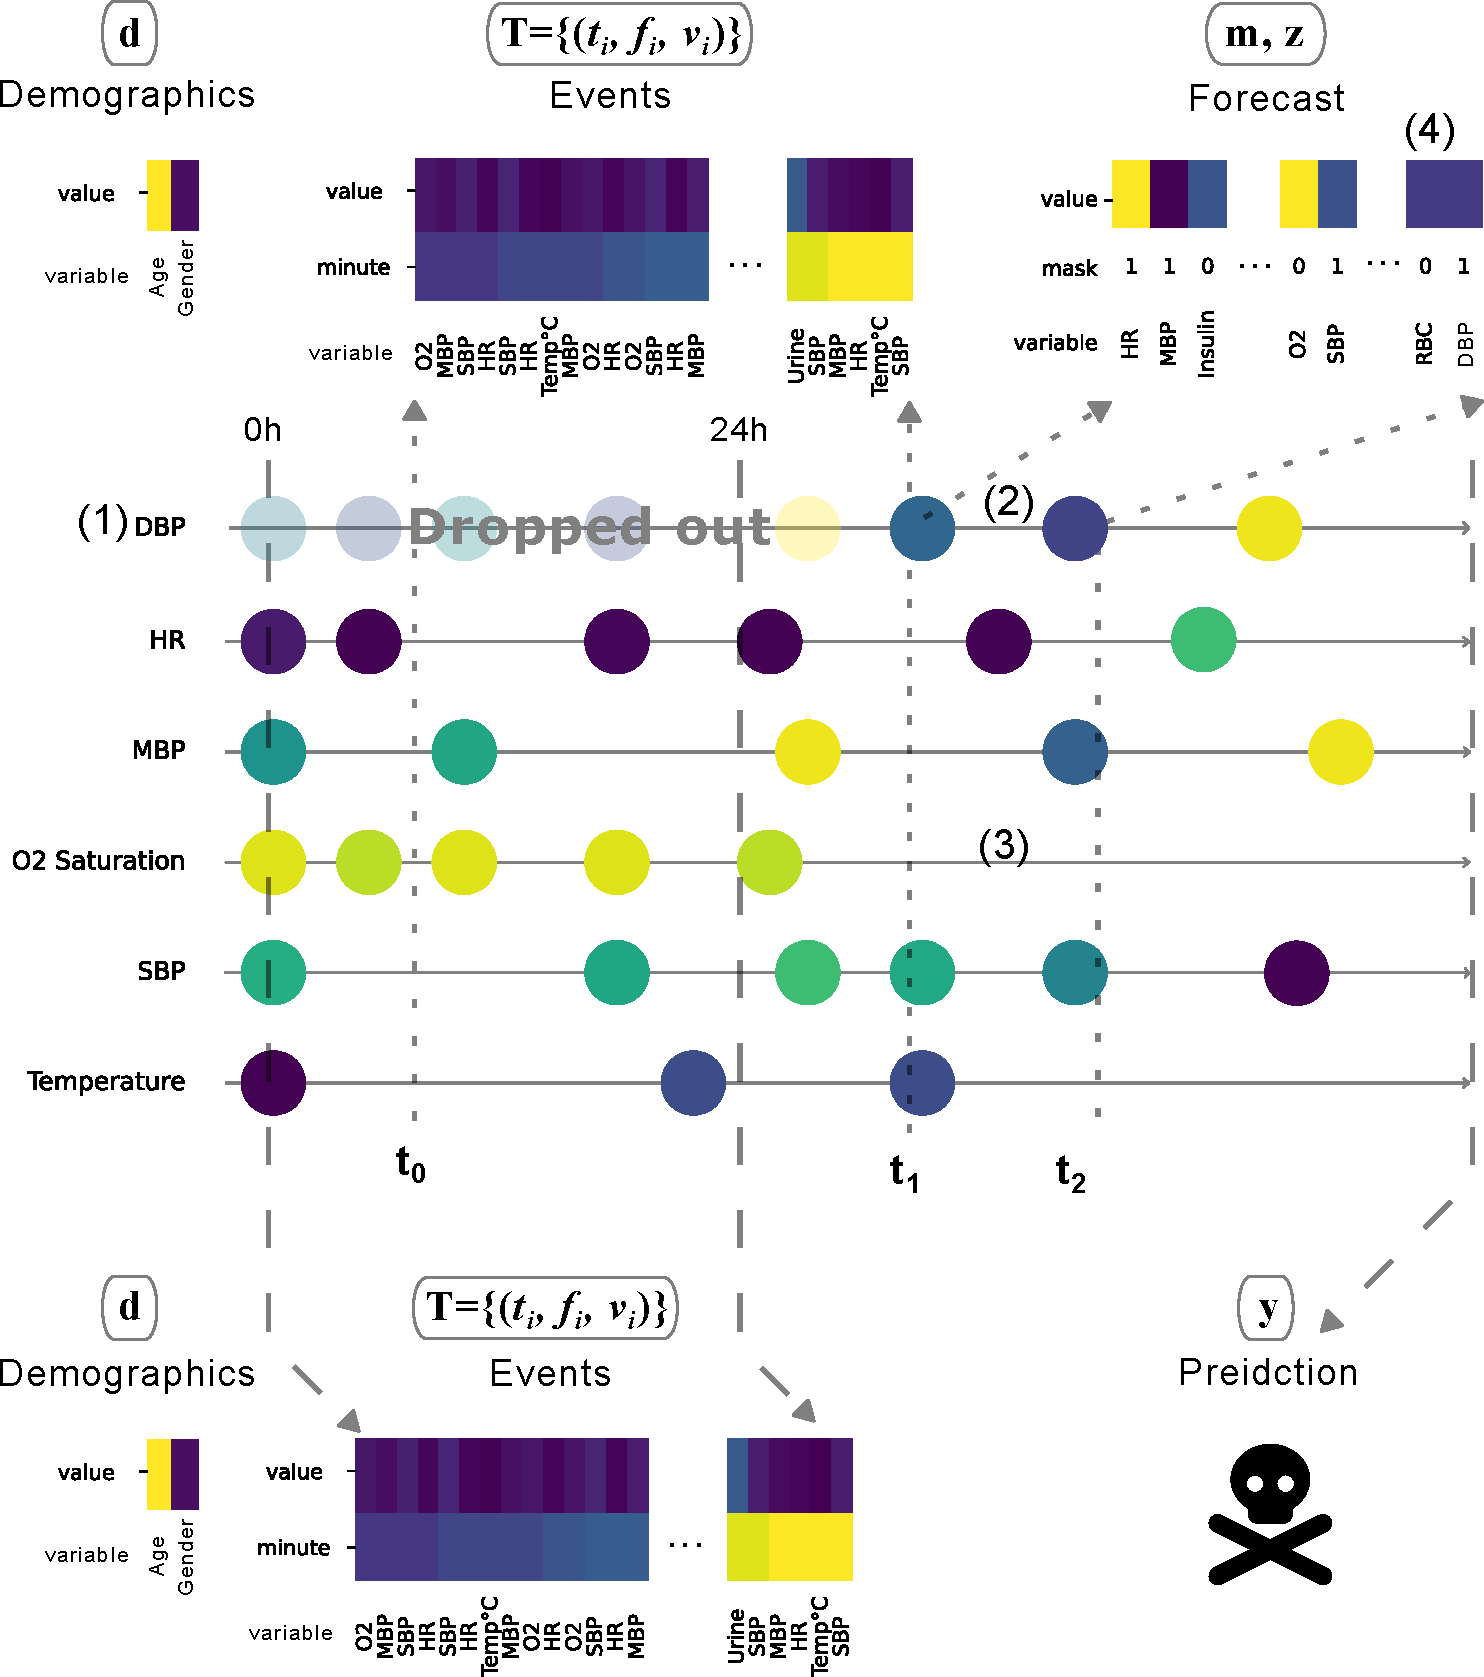
\includegraphics[width=\textwidth]{./figures/model_input}
    \caption{Visualization of the input structure for the forecasting and mortality prediction tasks.
    The DBP time series was excluded from input by a random variable dropout (1). Meanwhile  the mask for DBP has value 1 because it was observed in the data and participates in the forecast loss (2). The forecast mask for O2 Satuaration is 0 because it was not observed in the forecast window (3). RBC has mask 0 because it is not present in the observed data (4).}
    \label{fig:model_input}
\end{figure}

\subsection{Pretrained Model}

During the pretraining phase, the backbone model described in \cref{sec:backbone} is extended by adding a single-layer \gls{ffn} as a forecasting head \( \mathcal{M}_{pt}(\mathbf{d}_i, \mathbf{T}_i) = \mathbf{W}_f \cdot \mathcal{M} + \mathbf{b}_f = \hat{\mathbf{z}} \in \mathbb{R}^{|\mathcal{F}|} \) with parameters \( \mathbf{W}_f \in \mathbb{R}^{d \times \mathcal{F}|} \) and \( \mathbf{b}_f \in \mathbb{R}^{|\mathcal{F}|} \) that maps the integrated vector representation produced by a backbone network to a vector of feature value predictions. The detailed algorithm of pretraining phase is provided in \cref{algorithm:pretrain}.

This configuration is designed to perform a regression task, specifically forecasting future values of the time-series data. The goal of this phase is to pretrain the model, allowing it to learn temporal dynamics and generate robust embeddings that can be used for various downstream tasks.

% TODO: picture of heads

\subsection{Masked Mean Squared Error Loss}

The model's output vector covers all possible features. However, not all features may be observed in the given data. To avoid computing errors for unobserved features, we apply a masked \gls{mse} loss function, evaluating the prediction error only for the features observed within prediction timeframe. It calculates the average of the squared differences between the predicted values \(\hat{z}_i\) and the true values \(z_i\), for the observed features.

\begin{equation}
    \label{eq:mmse}
    \mathcal{L}_{\text{mMSE}}( \mathbf{z}, \hat{\mathbf{z}}, \mathbf{m}) = \frac{\mathbf{m}^\top \cdot (\hat{\mathbf{z}} - \mathbf{z})^{\odot 2}}{\|\mathbf{m}\|_1}  ,
\end{equation}

where

\begin{itemize}
\item \( \mathbf{m} \in {0, 1}^|\mathcal{F}|\) is the mask vector indicating which features were observed,
\item \( (\cdot)^{\odot 2} \) denotes element-wise squaring,
\item \( \|\mathbf{m}\|_1 \) is the sum of the elements of the mask vector (i.e., the number of non-masked values).
\end{itemize}

This formulation ensures that only predictions for observed features contribute to the loss calculation.


\begin{algorithm}[h]
\setstretch{1.35}
\caption{Model Pretraining}
\label{algorithm:pretrain}
\KwData{\( \mathcal{D}_{train},\mathcal{D}_{val},\mathcal{D}_{test} = \{(\mathbf{d}_i, \mathbf{v}_i, \mathbf{t}_i, \mathbf{f}_i)\}_{i=1}^{N} \) }
\KwResult{Pretrained model \(\mathcal{M}_{pt}\) with minimal validation loss \( \mathcal{L}^{val}_{mMSE} \)}

\textbf{Data Preparation:} \\
\nl Standardize feature values: \(\bar{v}_f = \frac{v_f - \mu_f}{\sigma_f}\) \;

\textbf{Training:} \\
\ForEach{epoch until validation loss \(\mathcal{L}^{val}_{mMSE} \) stops decreasing} {
    \nl Initialize accumulated loss \(\mathcal{L}_{acc} = 0\) \;
    \ForEach{\(i \in [1, N] \)} {
        \nl Sample input data: \( \mathbf{T}_{\qty{24}{\hour}} \) \tcp*[l]{see \cref{eq:input_24_window}} \label{alg:pretrain_epoch_start}
        \nl Apply variable dropout: \( \mathbf{T}'_{\qty{24}{\hour}} \) \tcp*[l]{see \cref{eq:variable_dropout}}
        \nl Compute target vector: \( \mathbf{z} \in \mathbb{R}^{|\mathcal{F}|} \) \tcp*[l]{see \cref{eq:forecast_target}}
        \nl Compute forecast mask: \(\mathbf{m} \in \{0, 1\}^{|\mathcal{F}|}\) \;
        \nl Forecast values: \(\hat{\mathbf{z}} = \mathcal{M}_{pt}(\mathbf{d}_i,\mathbf{T}'_{\qty{24}{\hour}}) \) \;
        \nl Accumulate loss: \(\mathcal{L}_{acc} \mathrel{+} = \mathcal{L}^{train}_{mMSE} (\mathbf{z}_i, \hat{\mathbf{z}}_i, \mathbf{m}) \) \tcp*[l]{see \cref{eq:mmse}} \label{alg:pretrain_compute_loss}
        \If{\(i \mod \text{batch size} = 0\)} {
            \nl Backpropagate and update model weights \;
            \nl Reset accumulated loss \(\mathcal{L}_{acc} = 0\) \;
        }
    }
    \nl Repeat \crefrange{alg:pretrain_epoch_start}{alg:pretrain_compute_loss} for \(\mathcal{D}_{val}\) and compute validation loss \(\mathcal{L}^{val}_{mMSE} \) \;
}
\textbf{Evaluation:} \\
\nl Repeat \crefrange{alg:pretrain_epoch_start}{alg:pretrain_compute_loss} for \(\mathcal{D}_{test}\) and compute test loss \(\mathcal{L}^{test}_{mMSE} \) \;
\end{algorithm}



\subsection{Summary of Pretraining Phase}

\begin{itemize}
    \item \emph{Task}: Time series forecasting.
    \item \emph{Data}: Demographics + random \qty{24}{\hour} time-series window without labels.
    \item \emph{Model}: Backbone model appended by a single-layer \gls{ffn} (forecast head).
    \item \emph{Loss}: masked Mean Squared Error loss.
    \item \emph{Learning type}: Self Supervised.
    \item \emph{Purpose}: Pretraining the model to learn temporal dynamics and generate useful embeddings for downstream tasks.
\end{itemize}

%%%%%%%%%%%%%%%%%%%%%%%%%%%%%%%%%%%%%%%%%%%%%%


\section{Fine-tuning Phase}
\label{sec:finetuning}

The fine-tuning phase involves adapting the pretrained model to specific downstream tasks, particularly binary classification tasks such as mortality prediction. In the mortality prediction, the model \( \mathcal{M}_{ft} \) must determine whether a patient is likely to survive based on data available within the first \qty{24}{\hour} of an \gls{icu} stay. Building upon the temporal dynamics learned during pretraining, the model is fine-tuned to optimize its performance for this specific supervised learning objective.

\subsection{Labeled Data}

Consider a labeled dataset \( \mathcal{D}' = \{(\mathbf{d}_i, \mathbf{T}_i, y_i)\}_{i=1}^{N'} \), where \(N'\) represents the number of labeled samples. Here, \( y_i \in \{0, 1\} \) is a binary label that indicates the patient's outcome, e.i. the mortality during the hospital stay. The number of labeled samples \( N' \) may be smaller than \( N \) due to the lack of additional labeled data. The model must accurately determine whether a patient is likely to survive based on the input data from the first \qty{24}{\hour} of the \gls{icu} stay so only a fraction of entire time series is selected, corresponding to using \( t_0 = 0 \) and \( t_1 = \qty{24}{\hour}\) in \cref{eq:normalize_time}. The time series is then defined as

\begin{equation}
    \label{eq:first_24_window}
    \mathbf{T}_{\qty{24}{\hour}} = \left\{ \left( \bar{t}_j, \, f_j, \, \bar{v}_j \right) \ \middle|\ t_j \leq \qty{24}{\hour} \right\}_{j = 1}^{n}.
\end{equation}

The bottom part of \cref{fig:model_input} illustrates the construction of inputs for the mortality prediction task. Similarly to the previous phase, the input structure consists of three vectors: the feature values \( \mathbf{v} \), the corresponding timestamps \( \mathbf{t} \), and the feature identifiers \( \mathbf{f} \), along with the demographics values \( \mathbf{d} \), but in contrast with the forecasting task the selected time series is always the first \qty{24}{\hour} of the \gls{icu} stay. Additionally, the binary label \( y \) is used to compute the loss during training.

\subsection{Fine-tuned Model}

During this phase, the pretrained forecasting model \(\mathcal{M}_{pt} \), as described in \cref{sec:pretraining}, is extended by adding a single neuron with a sigmoid activation function, thus acting as a classification head:
\[
    \mathcal{M}_{ft}(\mathbf{d}_i, \mathbf{T}_i) = \text{sigmoid}(\mathbf{W}_c \cdot \mathcal{M}_{pt}(\mathbf{d}_i, \mathbf{T}_i) + \mathbf{b}_c) = \hat{y}_i \in [0, 1]
\]

where \(\mathbf{W}_c \in \mathbb{R}^{|\mathcal{F}| \times 1}\) and \(\mathbf{b}_c \in \mathbb{R}\) are the layer weights and bias, respectively. The output \(\hat{y}_i\) represents the predicted probability of mortality for a given patient.

\subsection{Weighted Binary Cross-Entropy Loss}

\Gls{bce} is a loss function commonly used in binary classification problems where the target variable has two possible outcomes, \num{0} and \num{1}. It measures the performance of a classification model whose output is a probability value between \num{0} and \num{1}, indicating the likelihood of the positive class. In this study, the \gls{wbce} loss function is employed to address the issue of class imbalance by assigning a higher weight to the minority class. Before the fine-tuning process begins, the positive class proportion \(p\) is calculated as:

\[
p = \frac{1}{N} \sum_{i=1}^{N} y_i,
\]

where \(y_i \in \{0,1\}\) are the true labels, and \(N\) is the total number of samples. The positive class weight \(w\) is then defined as:

\begin{equation}
    \label{eq:positive_class_weight}
    w = \frac{1 - p}{p}.
\end{equation}

The \gls{wbce} loss is formulated as:

\begin{equation}
    \label{eq:wBCE}
    \mathcal{L}_{\text{wBCE}} = - \frac{1}{N} \sum_{i=1}^{N} \left[ w \cdot y_i \cdot \log(\hat{y}_i) + (1 - y_i) \cdot \log(1 - \hat{y}_i) \right],
\end{equation}

where \(\hat{y}_i \in [0,1]\) are the predicted probabilities of the positive class. By incorporating the weight \(w\), the loss function places more emphasis on correctly classifying instances of the minority class, thus improving the model's performance on critical outcomes.

This weighting ensures that the model does not become biased toward the majority class, which is particularly relevant in healthcare applications where the minority class often represents critical outcomes.

\begin{algorithm}[h]
\setstretch{1.35}
\caption{Model fine-tuning}
\label{algorighm:finetune}
\KwData{\( \mathcal{D}'_{train}, \mathcal{D}'_{val}, \mathcal{D}'_{test} = \{(\mathbf{d}_i, \mathbf{v}_i, \mathbf{t}_i, \mathbf{f}_i, y_i)\}_{i=1}^{N'} \) }
\KwResult{Fine-tuned model \(\mathcal{M}_{ft}\) with highest \gls{auroc}+\gls{aucpr} }

\textbf{Data Preparation:} \\
\nl Standardize feature values: \(\bar{v}_f = \frac{v_f - \mu_f}{\sigma_f}\) \label{alg:finetune_start}\;
\nl Select first 24 hours of \gls{icu} stay: \( \mathbf{T}_{\qty{24}{\hour}} \) \tcp*[l]{see \cref{eq:first_24_window}}
\nl Compute positive class weight: \(w\) \tcp*[l]{see \cref{eq:positive_class_weight}}

\textbf{Training:} \\
\ForEach{epoch until metrics stop improving} {
    \nl Initialize accumulated loss \(\mathcal{L}_{acc} = 0\) \;
    \ForEach{\(i \in [1; N']\)} {
        \nl Apply random variable dropout: \( \mathbf{T}'_{\qty{24}{\hour}} \) \tcp*[l]{see \cref{eq:variable_dropout}}
        \nl Predict class: \(\hat{\mathbf{y}}_i = \mathcal{M}_{ft}(\mathbf{d}_k, T'_{\qty{24}{\hour}} )\) \; \label{alg:finetune_prediction}
        \nl Accumulate loss: \(\mathcal{L}_{acc} \mathrel{+} = \mathcal{L}^{train}_{wBCE} (y_i, \hat{y}_i, w) \) \tcp*[l]{see \cref{eq:wBCE}} \label{alg:finetune_compute_loss}
        \If{\(i \mod \text{batch size} = 0 \)} {
            \nl Backpropagate and update model weights \;
            \nl Reset accumulated loss \(\mathcal{L}_{acc} = 0\) \;
        }
    }
    \nl Repeat \crefrange{alg:finetune_start}{alg:finetune_prediction} for \(\mathcal{D}'_{val}\) to get \(\hat{\mathbf{y}}_{val}\) \;
    \nl Compute \gls{auroc} and \gls{aucpr} for \(\hat{\mathbf{y}}_{val}\) \;
}
\textbf{Evaluation:} \\
\nl Repeat \crefrange{alg:finetune_start}{alg:finetune_prediction} for \(\mathcal{D}'_{test}\) to get \(\hat{\mathbf{y}}_{test}\) \;
\nl Compute \gls{auroc}, \gls{aucpr} and \gls{minrp} for \(\hat{\mathbf{y}}_{test}\) \;
\end{algorithm}


\subsection{Summary of Fine-tuning Phase}

\begin{itemize}
    \item \emph{Task}: Time series classification.
    \item \emph{Data}: Demographics + first \qty{24}{\hour} of time series.
    \item \emph{Model}: Pretrained model appended with a single neuron with sigmoid activation (mortality prediction head).
    \item \emph{Loss}: \glsentrylong{wbce}.
    \item \emph{Learning Type}: Supervised, mortality prediction.
    \item \emph{Purpose}: Adapt the pretrained model for binary classification tasks.
\end{itemize}

\section{Implementation Details}
\label{sec:implementation_details}

The model was implemented using PyTorch 2.4 with CUDA 12.1. More technical details, along with the model implementation and data-processing code, are available at \citeurl{thesiscode}. For the baseline models described in \cref{sec:baselines}, we utilized implementations from the repository at \url{https://github.com/sindhura97/STraTS}. The experiments were conducted on a desktop running Ubuntu 22.04 with \qty{64}{\giga\byte} of RAM, 16-threads AMD Ryzen 7 5800X CPU, a single NVIDIA GeForce RTX 3060 GPU with \qty{12}{\giga\byte} of memory, \num{112} Tensor cores and \num{28} Streaming Modules

\subsection{Model Compilation}

We leveraged the \texttt{torch.compile} feature in PyTorch to optimize computational efficiency. With minimal code modifications the \texttt{torch.compile} function enables just-in-time (JIT) compilation of PyTorch code into optimized CUDA kernels, significantly reducing Python overhead and improving runtime performance, particularly for GPU-based models.

\subsection{Mixed Precision Training}

We employed Automatic Mixed Precision (AMP) with the \texttt{bfloat16} format. The \texttt{bfloat16} is a 16-bit floating-point format that maintains a dynamic range similar to \texttt{float32}, which is beneficial for stable training while using less memory and computational resources on modern NVIDIA GPUs. AMP enables the use of mixed precision by dynamically selecting between \texttt{bfloat16} for operations where reduced precision is sufficient and \texttt{float32} where more precision is required. Moreover, the AMP allows using Nvidia Tensor Cores for faster computation, which are specifically designed for efficient matrix multiplication and convolution operations, providing the 8x theoretical throughput compared to standard CUDA cores.

%\subsection{Fused AdamW Optimizer}
%
%PyTorch provides fused implementations for certain optimizers, including Adam and AdamW. Fused optimizers combine multiple computational steps into a single CUDA kernel, reducing memory overhead and kernel launch latency. This leads to improved performance during training by making more efficient use of GPU resources.

\subsection{Efficient Attention}
\label{sec:efficient_attention}

We incorporated a highly optimized implementation of the attention mechanism from the \texttt{xFormers} library \cite{xFormers}. According to their experiments, under certain conditions, this implementation can be up to ten times faster than the standard PyTorch implementation. This performance gain is achieved through the use of optimized low-level GPU instructions and improved memory management. In our preliminary tests, we confirmed that this implementation significantly increased processing speed and reduced memory usage.

\subsection{Vectorized NumPy Operations}

We re-implemented data processing, batching, value normalization, and dropout functions used by the original \citefield{STraTS2022}{shorttitle} algorithm. We employed vectorized NumPy operations instead of explicit Python loops wherever possible. This approach minimizes the overhead associated with Python's interpreter and takes advantage of modern CPU architectures for parallel execution, resulting in significantly faster data processing.

This strategy allowed us to preprocess the data and generate batches of input data efficiently on a single CPU core, avoiding noticeable training startup delays and multithreading synchronization overheads. By eliminating the bottleneck caused by slow batch generation, we ensured that the GPU remained fully utilized throughout the training sessions.

\subsection{Other Modifications}
\label{sec:other_modifications}

% TODO: Double check if this all is still true

Based on our observations during the initial training runs we made several modifications to the model to enable the use of the Memory-Efficient Attention implementation \cite{MemoryEfficientAttention}, improve the model's computational performance and stability, and enhance the training process.

The original implementation of the \citefield{STraTS2022}{shorttitle} model limited the number of pretraining epochs to \num{30}. However, we observed that this was often insufficient to reach the lowest validation loss during pretraining. To address this issue, we allowed the model to train for unlimited number of epochs and rely on early stopping to prevent overfitting.

Furthermore, we reduced the number of attention heads from \num{16} to \num{8}, thereby increasing the dimension of each attention head from unconventionally small \num{4} to \num{8}. This change was necessary to utilize the optimized attention kernels described in \cref{sec:efficient_attention}, which require the size of the attention heads to be divisible by \num{8}. According to \href{https://developer.nvidia.com/blog/optimizing-gpu-performance-tensor-cores/}{NVIDIA's guidelines}, Tensor Cores are activated when the number of  parameters of a fully-connected layer is divisible by \num{8} for the \texttt{bfloat16} AMP computations.
By adjusting the model's parameters to align with these requirements, we enabled the use of Tensor Cores, resulting in significant performance improvements.

Additionally, we increased the validation and test batch sizes to \num{112}, allowing the batches to be evenly distributed among the available \num{112} Tensor Cores of our GPU. The entire validation and training datasets were loaded to the GPU memory to be reused across multiple cross-validation runs. This allowed to avoid I/O bottlenecks caused by data transfer between RAM and GPU memory and ensure that the GPU remains fully utilized during validation and testing. Furthermore, the data was sorted by sequence length to minimize batch padding and reduce the memory overhead associated with variable-length sequences. It worth noting that these optimizations should be used with caution, as it may introduce bias in batch composition and potentially hinder training. We applied this technique only during evaluation and testing phases, that do not affect the model's training process.

Lastly, we reduced the number of features from \num{129} to \num{128} by removing a single ``Lymphocytes (Absolute)'' feature, which had a very high percentage of missing values - only \num{303} observations of this clinical variable were found in the dataset. This change was made primarly to allow the number of features to be divisible by \num{8}, enabling more efficient use of GPU's Streaming Modules during the computation of the forecast head.


\subsection{Weights\&Biases integration}

Weights \& Biases (W\&B) \cite{wandb} is a tool for tracking machine learning experiments, providing functionalities for logging metrics, visualizing results, and sharing findings. We integrated W\&B into our experimental workflow to enhance experiment tracking, visualization, and reproducibility.

We utilized W\&B in the following ways:
\begin{itemize}
    \item \textbf{Aggregated Results}: W\&B allowed us to aggregate and visualize the results of training runs in a single dashboard, facilitating easy comparison across different experiments.
    \item \textbf{Real-Time Monitoring}: It enabled real-time monitoring of the training process, including loss, evaluation metrics, gradient norms, and other relevant parameters.
    \item \textbf{Performance Tracking}: Provided a convenient way to track and compare model performance across different hyperparameter settings and architectures.
    \item \textbf{Reproducibility}: Stored model checkpoints, logs, and metrics, ensuring reproducibility and allowing us to run additional tests without retraining the model.
\end{itemize}

Overall, the integration of W\&B significantly improved our ability to manage and analyze and reproduce our experiments, despite the initial integration challenges.

\section{Baseline Methods}
\label{sec:baselines}

To evaluate model performance, we replicated the comparative analysis conducted by \citeauthor{STraTS2022} using the following baseline models.
Additionally, we evaluated our own optimized implementation of the original \citefield{STraTS2022}{shorttitle} architecture.

We employed the hyperparameters and configurations provided in their repository, although these sometimes contradicted the details mentioned in the original paper. Specifically, while they reported using 4 attention heads and a hidden dimensionality of 32, the code used 16 attention heads and a hidden dimensionality of 64. By using the hyperparameters provided in the code, we obtained results consistent with the previous study (denoted as ``\citefield{STraTS2022}{shorttitle}'' in our results).

Lastly, we ran a subset of other baseline models provided in the paper's repository. The baselines were trained and evaluated on the same \gls{mimiciii} dataset, with some modifications to the input data format due to the architectural features of each model.

\subsection{Gated Recurrent Unit}

Gated Recurrent Unit (GRU) \cite{gru,gru-evaluation} is a type of Recurrent Neural Network (RNN) that uses gating mechanisms to capture temporal dependencies in sequential data. Unlike traditional RNNs, GRUs address the vanishing gradient problem by adaptively controlling the flow of information through update and reset gates, allowing the model to capture dependencies of different time scales without the need for separate memory cells, as in Long Short-Term Memory (LSTM) networks.

The GRU processes the input matrix sequentially, aggregating information from long sequences into a single vector representation of the entire time series for the following mortality prediction.

\subsection{Gated Recurrent Unit with Decay}

GRU with Decay (GRU-D) \cite{GRUD2018} extends the standard GRU architecture to handle missing data and irregular time intervals, which are common in clinical time-series data. GRU-D introduces trainable decay mechanisms that adjust the hidden state and input features based on the time elapsed since the last observation for each feature.

The model decays both the input features and the hidden state toward their empirical mean values over time, allowing it to learn patterns in the presence of missing data and irregular sampling intervals. GRU-D was originally applied to the \gls{mimiciii} dataset for mortality prediction and \gls{icd}-9 diagnosis prediction, demonstrating state-of-the-art performance in handling informative missingness in clinical time-series data.

\subsection{Temporal Convolutional Network}
Temporal Convolutional Network (TCN) \cite{tcn} is a convolutional neural network architecture designed for sequence modeling tasks. TCN employs dilated causal  (``meaning that there is no information leakage from future to past'') convolutions and residual connections to capture long-range temporal dependencies while maintaining computational efficiency. Dilated convolutions enable the network to have ``an exponentially large receptive field'', allowing it to model dependencies over long sequences without a significant increase in computational cost.

The residual connections in TCN help mitigate the vanishing gradient problem, improving the training of deep networks. TCNs also offer advantages in parallelism and flexible receptive field size compared to recurrent architectures, making them a competitive choice for sequence modeling.

\subsection{Simply Attend and Diagnose}

Simply Attend and Diagnose (SaND) \cite{SAND2018} is a model specifically designed for clinical time-series data, utilizing a transformer-based architecture with causal self-attention mechanisms. SaND replaces recurrent computations with attention mechanisms, allowing for parallel processing of sequences and mitigating the inefficiencies associated with RNNs, especially for long sequences.

To handle variable-length sequences and irregular sampling, SaND relies on a dense interpolation that creates a fixed-length representation of the input data. The causal self-attention ensures that at each time step, the model only attends to previous time steps, preserving the temporal ordering of observations. Using the \gls{mimiciii} dataset SaND has demonstrated state-of-the-art performance on several tasks including mortality prediction, length of stay forecasting, and others.

\subsection{Input Data Representation}

The input for the GRU, TCN, and SaND models is a time-series matrix \(M \in \mathbb{R}^{T \times |\mathcal{F}|}\) with hourly aggregation, where \(T\) is the maximum time (e.g., \qty{24}{\hour}), and \(|\mathcal{F}|\) is the number of features. Missing features are imputed with mean values computed for the corresponding \gls{icu} stay and feature. Additionally, the time since the previous observation of each feature and a boolean missingness indicator are included as extra features at each time step to provide the models with information about temporal gaps in the data.

The GRU-D model processes sequences differently. The GRU-D cell takes a sequence of feature values \(M \in \mathbb{R}^{n \times |\mathcal{F}|}\) along with missingness indicators and time since the last observation at each time when one or more measurements are observed, where \(n\) is the number of observations, limited to \num{880} to match the constraints of the \citefield{STraTS2022}{shorttitle} model.

For all the baseline models, we used an approach identical to that of our studied model, described in \cref{sec:demographics_embedding}, to compute the demographics embedding \( \mathbf{e}^d \) with dimensionality \( d = 64 \). This embedding is then concatenated to the time-series vector representation generated by the corresponding baseline model. The final layer (the head) is identical across all models and consists of a single output neuron with a sigmoid activation function for mortality prediction, as described in \cref{sec:finetuning}. The hyperparameters for all models along with the number of trainable parameters \footnote{The number of trainable parameters of \citefield{STraTS2022}{shorttitle} model is smaller than ``Ours'' due to the exclusion of the layer normalization parameters. Although the layer normalization was mentioned in the original paper, for unknown reasons it was commented out (disabled) in the corresponding source code.} can be found in \cref{tab:hyperparams}.



\begin{table}
\centering
\caption{Hyperparameters used in the experiments for all models along with the number of trainable parameters.}
\begin{tabular}{lll}
\toprule
\textbf{Model} & \textbf{Hyperparameters} & \textbf{Parameters num.} \\
\midrule
GRU & LR = 5e-4 & 95,745 \\
GRU-D & LR = 5e-4 & 79,363 \\
TCN & LR = 5e-4, layers = 4, filters = 64, kernel size = 4 & 248,385 \\
SAnD & LR = 5e-4, N = 4, r = 24, M = 12, h = 2, he = 8 & 167,457 \\
STraTS & LR = 5e-4 \& 5e-5, M = 2, h = 16 & 104,867 \\
Ours & LR = 5e-4 \& 5e-5, M = 2, h = 8 & 105,185 \\
\midrule
\multirow{4}{*}{\textbf{Common}}
& Dropout 0.2 \\
& Hidden dim. 64 \\
& Batch size 16 \\
& Gradient clipping 0.3 \\
& Max number of observations 880 \\
\bottomrule
\end{tabular}

\label{tab:hyperparams}
\end{table}

\section{Experiments}
\label{sec:experiments}

In this section, we present a series of experiments designed to evaluate the performance of our model and investigate various factors that may influence its effectiveness. We focus on issues such as class imbalance and data normalization techniques. Each experiment is conducted under controlled conditions to isolate the impact of the variable being tested.

In all experiments employ a 10-fold cross-validation approach, with results reported as mean performance metrics and standard errors. For the fine-tuning stage, we follow a setup consistent with the original study, training the model on randomly sampled data fractions ranging from \qtyrange{10}{100}{\percent} of the full training and validation labeled datasets. The test dataset remains consistent across all experiments to ensure comparability of results.



\subsection{Experiment 1: Addressing Class Imbalance}

Class imbalance is a common issue in binary classification tasks, where the number of samples in one class significantly outweighs the other \cite{LearningImbalancedData2009}. In our case, the positive class (mortality) is less frequent than the negative class (survival), which can lead to biased model predictions favoring the majority class. To address this issue, we experimented with different strategies to balance the training dataset and evaluated their impact on model performance.

Even when using a \gls{wbce} loss, there is a substantial chance that no positive samples will appear in a given mini-batch, rendering the class weights ineffective during those iterations. Let \( p \) denote the prevalence of the positive class (mortality rate) in the dataset, and \( B \) be the batch size. The probability \( P \) of having no positive samples in a batch is:

\[
P = (1 - p)^{B}.
\]

Substituting \( p = \num{\SupervisedTrainDeathPrevalence} \) (the mortality rate in train dataset) and \( B = 16 \), we obtain:

\[
P = (1 - 0.114)^{16} \approx 0.144 \approx \frac{1}{7}.
\]

This calculation shows that there is approximately a \qty{14}{\percent} chance that a batch contains no positive samples. In the absence of positive samples, the increased class weight has no effect during loss computation, as there are no positive instances to contribute to the loss. Consequently, the optimization steps during these iterations may shift the model towards predicting only the negative class, potentially leading to poor generalization. Similar computation for a smaller batch size of \( B = 4 \) yields a probability of approximately \qty{62}{\percent}, indicating that the issue becomes more pronounced with smaller batch sizes.

% TODO: proofread the following paragraph
An alternative to using a weighted loss is to perform random oversampling of the positive class with replacement, ensuring an equal number of positive and negative samples during each training epoch.  However, oversampling can increase the risk of overfitting to the duplicated positive samples \cite[][1267]{LearningImbalancedData2009}. We conducted experiments using this method as well to compare its performance with the class weighening.

\subsubsection*{Impact of Gradient Clipping}
\label{sec:clipping}

Gradient clipping is a technique used to prevent exploding gradients by scaling them when they exceed a certain threshold \cite[][409]{Goodfellow-et-al-2016}. In the original implementation of the model, a gradient clipping threshold of \num{0.3} was used. Although this detail was not explicitly mentioned in the original paper, it could significantly affect the model's performance, particularly in scenarios involving class imbalance.



Upon reviewing the gradient magnitudes in the W\&B logs, we observed that the gradients of several model parameters frequently exceeded the clipping threshold. When class weights are employed to address class imbalance, the loss associated with positive samples is multiplied by a larger weight to emphasize their contribution. However, if the resulting gradients exceed the clipping threshold, they are scaled down to the threshold value. This clipping reduces the intended effect of the increased class weights, as the gradients for positive samples are no longer proportionally larger than those for negative samples.

This issue becomes more pronounced with smaller batch sizes and as a result, may hinder the model's ability to learn effectively from the minority class. To test this hypothesis, we conducted experiments with varying batch sizes and with or without gradient clipping. We performed the following experiments to investigate the impact of class imbalance on model performance:

\begin{itemize}
    \item $\beta_{16}$ : Using regular (unweighted) \gls{bce} loss without any data resampling and a batch size of \( 16 \).
    \item $\beta_{16} + os$: Using unweighted \gls{bce} loss with random oversampling of the positive class to achieve a 50/50 class balance during training, with batch size of \( 16 \). The oversampling with replacement was performed only on the training split.
    \item $\beta_{16} + w + c$: Using weighted loss (\gls{wbce}) with a batch size of \( 16 \) and gradient clipping at  \( 0.3 \) (baseline).
    \item $\beta_{4} + w$: Using \gls{wbce} loss with a smaller batch size of \( 4 \).
    \item $\beta_{4} + w + c$: Using \gls{wbce} loss with a batch size of \( 4 \) and gradient clipping at \( 0.3 \).
\end{itemize}
In addition to the performance metrics discussed previously, we will calculate the average predicted probability of mortality for each experiment and compare it with the observed prevalence of mortality in the test dataset (\num{\SupervisedTestDeathPrevalence}). The difference between these values will be reported as the Mean Relative Error (MRE), which serves as an indicator of model calibration. This metric allows us to assess whether the model's risk estimates accurately reflect the true probability of mortality. By comparing predicted probabilities to the observed mortality prevalence, we can identify potential biases or shifts in the model's predictions. The metric is defined as:

\begin{equation}
    \label{eq:mre}
    MRE = \frac{1}{N} \sum_{i=1}^{N} \frac{\hat{y}_i - y_i}{y_i},
\end{equation}

where \( \hat{y}_i \) is the predicted probability of mortality for the \( i \)-th sample, \( y_i \) is the true label, and \( N \) is the total number of samples. Given the true mortality rate, the MRE values are bounded between \num{-1} and \num{7.764}, where MRE of \num{0} would indicate perfect alignment between the model's predicted risk scores and the true mortality rate, meaning that, on average, the predicted probabilities closely match the actual prevalence.

\subsection{Experiment 2: Data Normalization with ECDF Transformation}

The \citefield{STraTS2022}{shorttitle} model with its direct continuous value embeddings is an appropriate candidate to test our hypothesis about \gls{ecdf} transormation. Since the model employs a single \gls{cve} component to produce embeddings for continuous values across all features, it may encounter challenges in generating robust vector representations for observations with different distributions. Applying the \gls{ecdf} normalization method could potentially improve the model's performance and generalization capabilities by standardizing the value distributions across features\cite{emmert2022mathematical}.

The \gls{ecdf} is defined as

\[
    \hat{F}_n(x) = \frac{1}{n} \sum_{i=1}^{n} \mathbf{1}(X_i \leq x),
\]

where \(n\) is the total number of data points, \(X_i\) are the observed values, and \(\mathbf{1}\) is the indicator function, which equals \(1\) if \(X_i \leq x\) and \(0\) otherwise. This transformation maps each observed value to its corresponding percentile, thereby providing a uniform distribution of values in the range \([0, 1]\) across the feature space. An example of the \gls{ecdf} transformation for the feature ``Bilirubin (Total)'' is shown in \cref{fig:transforms_bilirubin}.

\begin{figure}
    \centering
    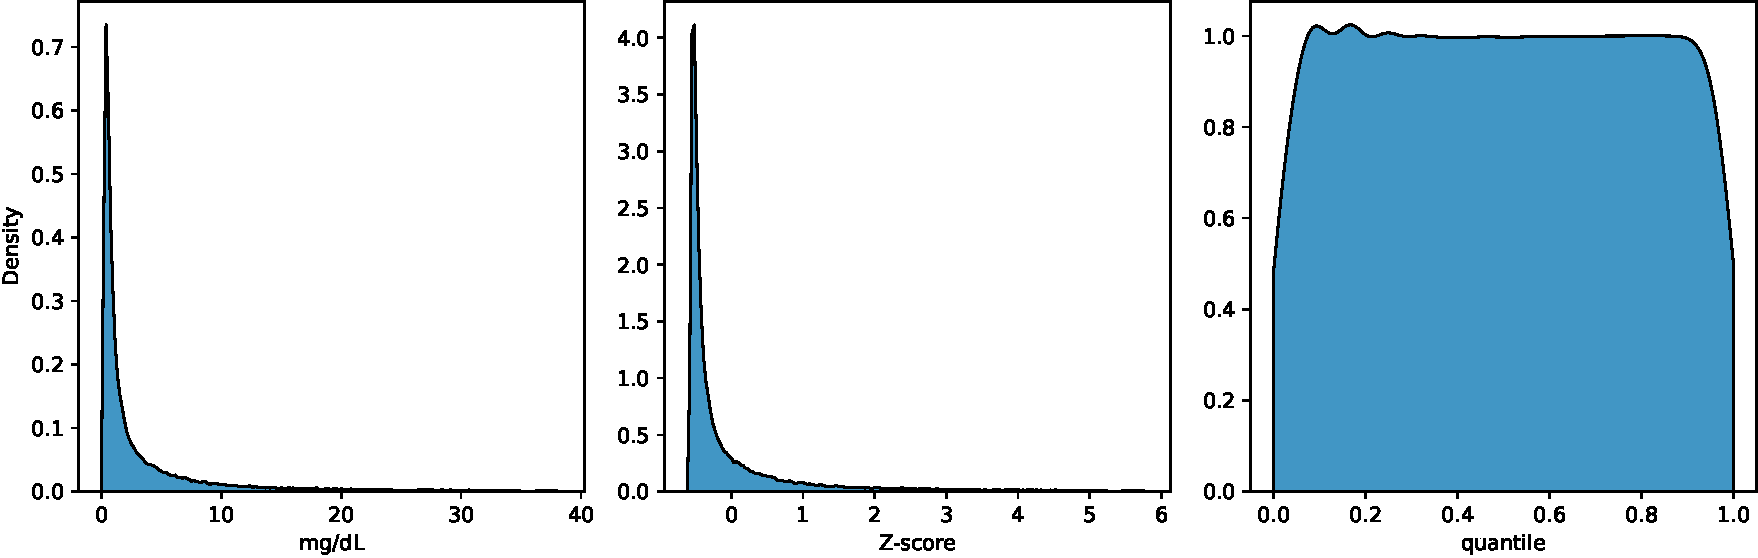
\includegraphics[width=\textwidth]{./figures/transforms_Bilirubin__Total_}
    \caption{KDE-plot of Z-score and \gls{ecdf} normalized distribution for the ``Bilirubin (Total)''  feature in the \gls{mimiciii} dataset. The \gls{ecdf} normalization provides a uniform distribution of values.}
    \label{fig:transforms_bilirubin}
\end{figure}



\subsubsection*{Model Architecture Changes}

The transformation to a bounded space between 0 and 1 allows us to use a sigmoid activation function in the forecasting head, which can be beneficial for the model training process by ensuring outputs are within the desired range.

The model is thus defined as follows:

\[
\mathcal{M}_{\text{ECDF}}(X) = \sigma(\mathcal{M}_{pt}(X)),
\]

where \(\sigma\) is the sigmoid function.

For the fine-tuning phase, we remove the final sigmoid activation layer used during pretraining. We transfer the pretrained model weights and add a single prediction neuron with a sigmoid activation function, following a similar procedure as described in \cref{sec:finetuning}. Thus, the resulting model architecture for a fine-tuning stage is identical to the original model.

\subsubsection*{Additional Considerations for Pretraining Model Evaluation}


\begin{figure}[h!]
    \centering
    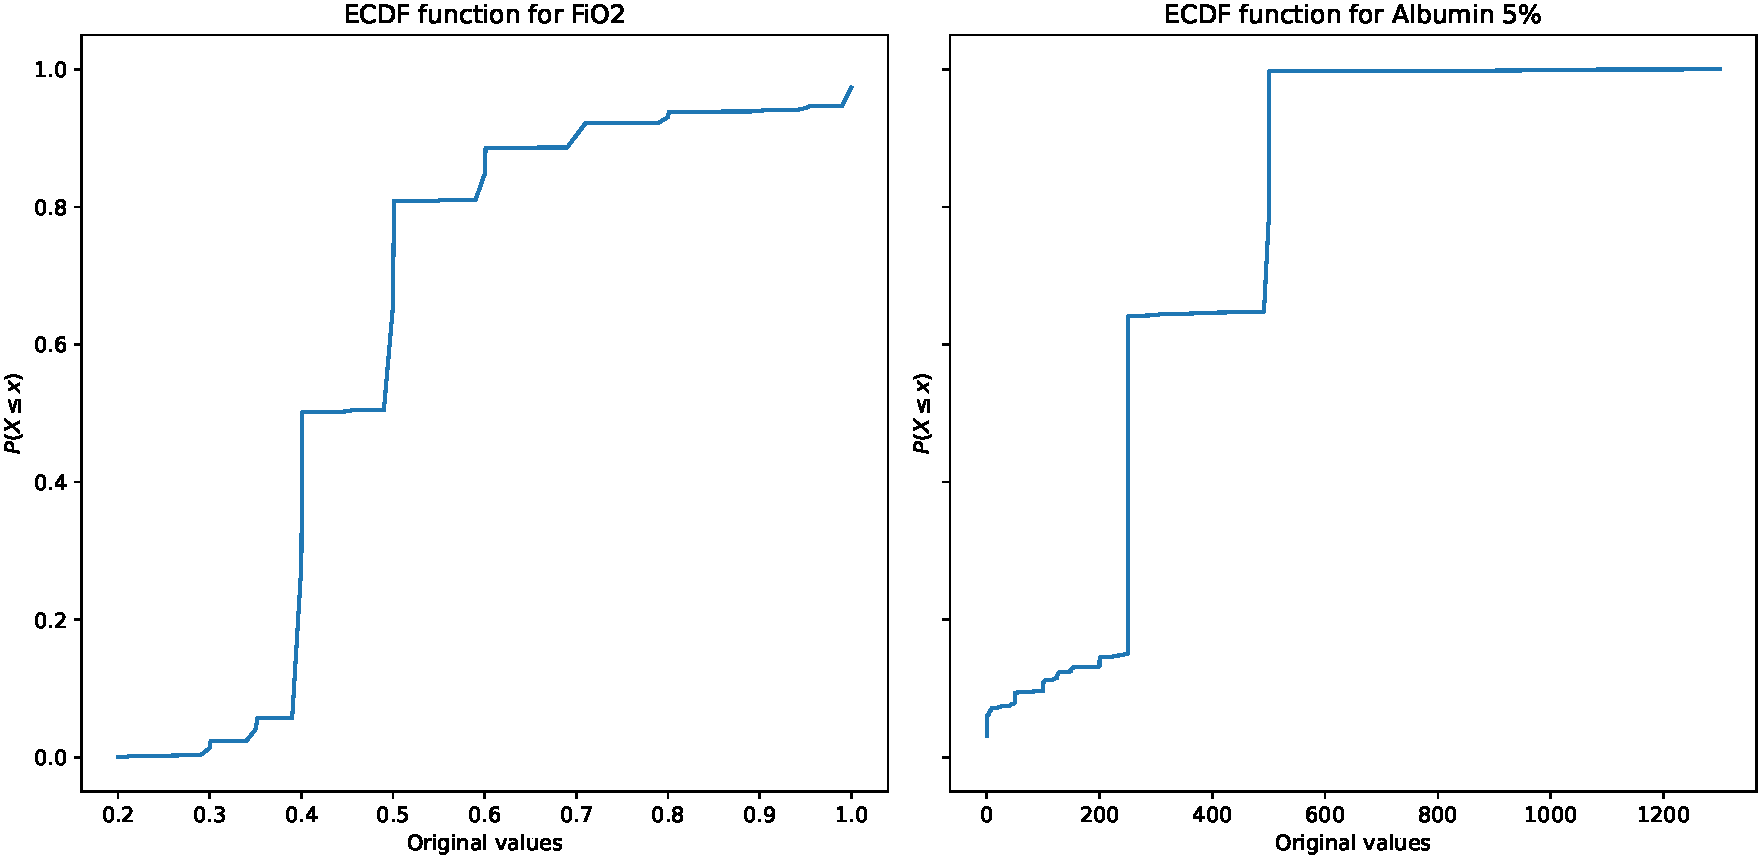
\includegraphics[width=\textwidth]{figures/ecdfs}
    \caption{\gls{ecdf} functions for variables with a low number of unique values, demonstrating the step-like nature of the \gls{ecdf} in such cases.}
    \label{fig:ecdf_pathological}
\end{figure}

When comparing the performance of models using Z-score and \gls{ecdf} normalizations during pretraining, the validation losses cannot be directly compared due to the differing value domains. To enable a fair comparison, we apply inverse transformations to the predicted values to return them to the original data domain. Subsequently, we reapply both Z-score and \gls{ecdf} normalizations to these predicted values and compute the corresponding losses, reported in the ``Z-score'' and ``ECDF'' columns of \cref{tab:normalization_experiments_pretrain}.

For the model trained with \gls{ecdf} normalization, we perform an inverse \gls{ecdf} transformation on its predictions for the test split, converting them back to the original variable domain. This allows us to compute the Z-score normalized values for both the true and predicted data, after which we can calculate the Mean Squared and Absolute errors in Z-score domain.

Conversely, for the model trained with Z-score normalization we apply the inverse Z-score transformation to its predictions, followed by the \gls{ecdf} transformation. This maps the predicted values to their corresponding quantiles using the \gls{ecdf}, allowing us to calculate the \gls{ecdf} \gls{mae} and \gls{ecdf} \gls{mse} between the predicted and true quantiles.

However, the step-function nature of the \gls{ecdf} presents challenges, particularly for variables with a limited number of unique values. Since the \gls{ecdf} increases by a step size \( s = \frac{n_v}{N} \) at each observed value \( v \), where \( N \) is the total number of data points and \( n_v \) is the frequency of \( v \), it may not adequately represent such variables. Discrete measurements like ``Albumin 5\%'' or low-precision variables such as ``FiO2'', which ranges from \num{0} to \num{1} in increments of \num{0.1}, are not well captured by the step-function nature of the \gls{ecdf}. The \gls{ecdf} functions for these cases are shown in \cref{fig:ecdf_pathological}.

Therefore, using the \gls{ecdf} directly for the inverse transformation can lead to inaccuracies. If the predicted value \( \hat{y} \) falls within the same step as the true value \( y \), the difference \( F(\hat{y}) - F(y) \) becomes zero, underestimating the error. Conversely, if the test dataset contains values not observed during training, the inverse transformation may overestimate the error, as those values cannot be accurately recovered from the model's predictions.

To address these issues and achieve a smoother transformation, we apply linear interpolation to \gls{ecdf}. This approach provides a continuous and monotonically increasing function, allowing for a more accurate transformation of predicted values, including those not present in the training dataset.

Given a sorted sequence of values \( V = \{v_1, v_2, \dots, v_N\} \) and their corresponding \gls{ecdf} values \( F(v_i) \), the interpolated \gls{ecdf} \( F(v) \) for any \( v \) between \( v_i \) and \( v_{i+1} \) is estimated as:

\[
F(v) = F(v_i) + \left( \frac{F(v_{i+1}) - F(v_i)}{v_{i+1} - v_i} \right) (v - v_i).
\]

This interpolation mitigates the limitations caused by the discrete nature of the \gls{ecdf} for variables with a limited number of unique values, ensuring more accurate error estimation during model evaluation.

\subsubsection*{Experiment Setup}

We conducted the following set of experiments to evaluate the impact of \gls{ecdf} normalization and different loss functions on the model performance:

\begin{itemize}
    \item \textbf{Z-score}: Using Z-score normalization;
    \item \textbf{ECDF}: Using \gls{ecdf} normalization.
\end{itemize}

In each experiment, we pretrain the model using the specified normalization method with identical \gls{mse} loss function, followed by fine-tuning for the downstream task of mortality prediction. We then evaluated the models to determine how these variations affected overall performance, particularly in terms of Mean Absolute and Squared Errors in both transformed data domains.

To improve the pretrained model evaluation, which involves random input window selection, we selected a random \qty{24}{\hour} window from each \gls{icu} stay in the test split \num{50} times and stored the resulted dataset in persistent storage. This approach allowed to reduce variability across test runs, resulting in more accurate and consistent estimates of model performance, ultimately providing a more reliable assessment of expected error. As before, we run the pretraining \num{10} times on all available training data. Then we fine-tune a pretrained model with the lowest validation loss for \num{10} folds on the data fractions from \qtyrange{10}{100}{\percent}.

\subsection{Experiment 3: Assessing Robustness to Noise and Outliers}

The \gls{mse} loss function is known for its sensitivity to large errors, which can cause the model to focus on reducing significant deviations. This characteristic may lead the model to disproportionately prioritize extreme values, potentially at the cost of overall performance for more typical values. In datasets with skewed distributions or outliers, such as clinical measurements that may exhibit extreme values without corresponding clinical significance, the \gls{mse} loss may encourage the model to overfit these rare occurrences.
% We will investigate the MSE by looking at the disttibution of loss

% TODO: "due to smaller magnitude of values" - double check if I actually stated this in the text
To validate our hypothesis about the improved robustness to noise due to the smaller magnitude of values, we conducted experiments designed to assess its performance under increasingly challenging data conditions.

\subsubsection*{Experiment Setup}

\paragraph{Inclusion of Outliers}

We generated new datasets without outlier filtering to obtain real-world data without the removal of outliers. This includes \num{6470} observations that were previously removed (\qty{0.008307}{\percent} of all data) and \num{81\,730} observations that were replaced with the median value (\qty{0.104929}{\percent} of all data), as described in \cref{sec:outlier-processing}.

\paragraph{Noise Injection}

Given the limited presence of outliers in the data and the model's current predictive performance of nearly \qty{90}{\percent} (as will be seen in the upcoming chapter), suggesting that the task may not be very challenging, we introduced additional noise to further assess the model's robustness. Specifically, we added the following types of noise to the dataset:

\begin{itemize}
    \item \qty{25}{\percent}, \qty{50}{\percent}, \qty{75}{\percent} and \qty{100}{\percent} Uniform Noise: We replaced a fraction of the individual observation values with random values drawn from a continuous uniform distribution bounded by each feature's \(f\) minimum and maximum  values observed in the entire dataset.
    \begin{align*}
        & \epsilon_f \sim \mathcal{U}(\min(\mathcal{F}_f), \max(\mathcal{F}_f)); \\
        & v'_f = v_f \cdot (1 - r) + \epsilon_f \cdot r, \\
        & \text{where } r \sim \text{Bernoulli}(p), \quad p \in \left\{\frac{1}{4}, \frac{2}{4}, \frac{3}{4}, 1\right\}.
    \end{align*}
    This type of noise is designed to simulate errors during measurements or data entry, which can occur in busy clinical settings with high workload conditions or attributed to input error in case of self-reported data.
    \item $1\sigma$, $2\sigma$, and $3\sigma$ Gaussian noise: We added Gaussian noise to all observed values, with standard deviations equal to one, two and three times the standard deviation of each feature's distribution \(\ sigma_f \), respectively:
    \begin{align*}
       & \epsilon_f \sim {\mathcal{N}}(0, (n\sigma_f)^{2}), \quad \text{where } n \in \{1, 2, 3\}; \\
       & v'_f = v_f + \epsilon_f.
    \end{align*}

    Consequently, this setup allows us to observe the model's resilience to measurement errors of varying magnitudes, which could represent different levels of clinical variability or measurement precision in real-world scenarios.
\end{itemize}

We expect that as noise levels increase, model performance will degrade, with uniform noise likely posing a greater challenge due to the presence of extreme values and removing the original data. This experiment will assess the model's resilience to such perturbations, providing insights into its robustness in clinical scenarios with potential measurement variability. Throughout this process, the initial patient splits were preserved to ensure that any observed changes in model performance could be attributed solely to the introduced noise and not to variability in the training or validation data.


\subsection{A Note on the \qty{100}{\percent} Noise Experiment}
\label{sec:100_noise}

In the experiment where \qty{100}{\percent} of the observation values \(v_i\) are replaced with noise, the model performance is expected to remain significantly above random chance, which may initially seem surprising. However, this can be explained by considering that the model's input data comprises multiple types of information, including time-series data \(\mathbf{T} = \{(t_i, f_i, v_i)\}_{i=1}^n\) and demographic data \(\mathbf{d} \in \mathbb{R}^D\). Among these, only the observation values \(v_i\) were randomized in the noise experiment, while the other components remained unchanged.

The inclusion of demographic variables, such as gender and, especially, age, holds substantial predictive power and was not randomized, as these variables are not typically subject to noise. Moreover, the presence of certain clinical measurements can signal severe conditions regardless of their specific values. For example, the administration of medications such as ``Epinephrine'' is often associated with cardiac arrest or severe hypotension, while indicators such as ``Norepinephrine,'' ``Dopamine,'' and ``Vasopressin'' suggest septic shock. Similarly, an ``Intubated'' status and ``FiO2'' levels are related to mechanical ventilation.

Additionally, the size of the available feature space and the number of observations recorded within a certain time window may further contribute to the model's predictive power. The model may learn patterns from the timing and frequency of observations or from the presence of specific features, even when the actual values are randomized.


For the \gls{ecdf} transformation, the uniformly distributed noise values are mapped to random values uniformly distributed between 0 and 1. Similarly, for the Z-score transformation, the uniformly distributed values in the range \( [a, b] \) are shifted to have a mean of 0 and scaled by their standard deviation.

The mean and standard deviation of a uniform distribution \( \text{Unif}(a, b) \) are given by:

\[
    \mu = \frac{a + b}{2}, \quad \sigma = \frac{b - a}{\sqrt{12}}.
\]

Applying the Z-score transformation to the uniform distribution yields the following:

\[
    Z(X) = \frac{X - \mu}{\sigma} = \frac{X - \frac{a + b}{2}}{\frac{b - a}{\sqrt{12}}} = \sqrt{12} \left( \frac{X - \frac{a + b}{2}}{b - a} \right).
\]

Since \( X \) follows \( \text{Unif}(a, b) \), the term \( \frac{X - \frac{a + b}{2}}{b - a} \) is uniformly distributed between \(-0.5\) and \(0.5\). Therefore, the transformed variable \( Z(X) \) becomes:

\begin{equation}
    \label{eq:uniform_z_range}
    Z(X) = \sqrt{12} \cdot \text{Unif}(-0.5, 0.5) = \text{Unif}\left( -\frac{\sqrt{3}}{1}, \frac{\sqrt{3}}{1} \right) \approx \text{Unif}(-1.732, 1.732).
\end{equation}

This result shows that the Z-score transformation of uniformly distributed noise results in another uniform distribution over a fixed range, similar to the \gls{ecdf}-transformed noise. Since both normalization methods transform the noise into standardized forms that do not convey meaningful predictive information, the model performance under \qty{100}{\percent} noise is expected to be similar for both methods.



\section{Chapter Conclusion}

In this chapter, we detailed the architecture and training procedures of our proposed model, including the backbone network, pretraining and fine-tuning phases, evaluation metrics, and implementation specifics. We also discussed the baseline methods used for comparison and outlined the experiments designed to assess various aspects of model performance. The methodologies presented lay the groundwork for the results and analysis in the subsequent chapter.

